\subsection{Stabilizer Configuration}

\begin{table}[!h]
    \centering
    \caption{Stabilizer Dimensions}
    \begin{tabular}{|c||c|c|c|} \toprule
        \textbf{Description} & {\textbf{Horizontal Stabilizer}} & 
        {\textbf{Vertical Stabilizer}} & \textbf{Units}\\ \midrule \hline
        AR & 4.5 & 1.5 & $\sim$ \\ \hline
        b (\textit{span}) & 67 & 27 & ft \\ \hline 
        $s_{\text{wing}}$ (\textit{area}) & 1,000 & 500 & ft$^2$ \\ \hline
        c/4 Sweep & 35 & 35 & degree \\ \hline
        $\lambda$ & 0.35 & 0.35 & $\sim$ \\ \hline
        Chord Root & 265.01 & 324.58 & in \\ \hline
        Chord Tip & 92.76 & 113.60 & in \\ \hline   
        Mean Aerodynamic Chord & 192.71 & 236.02 & in \\ \bottomrule
    \end{tabular}
    \label{tab:wingsizing}
\end{table}

Both the horizontal stabilizer \hl{edit out early stages etc} and vertical stabilizer are at very early stages in sizing.  Location of the stabilizers, as notated as the distance between the $\text{MAC}_{\text{wing}}$ and $\text{MAC}_{\text{stabilizers}}$, is likely to change after further stability analysis.

\subsubsection{Horizontal Stabilizer}
SAM Mk I uses a standard tail configuration.  The horizontal stabilizer is initially sized to be 25\% of $S_{wing}$.  This provides a starting point from which to begin stability analysis.  Use of an inverted NASA SC(2)-0412 airfoil for the horizontal stabilizer is proposed to provide a counter moment to the lifting effects of the wing.
\begin{figure}[!h]
    \centering
    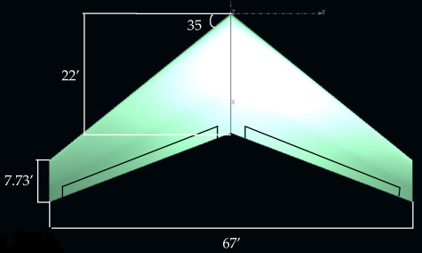
\includegraphics[width=0.75\textwidth]{Photos/stab/htail.png}
    \caption{Horizontal Stabilizer Top View}
    \label{fig:htailstab}
\end{figure}

\subsubsection{Vertical Stabilizer}
The vertical stabilizer is sized to be approximately 12.5\% of $S_{wing}$.  Additional attention must be directed at the vertical stabilizer to ensure directional stability.

\subsection{Control Surfaces}
Several control surfaces are built into the wing, horizontal stabilizer, and vertical stabilizer.  The main wing contains a flap mechanism from spanwise locations $11.5$ ft to $69.1$ ft and deflects a maximum of $\delta_F = 30\degree$.  An initial aileron sizing has determined potential placement from $72$ ft to $90$ ft.  The aileron deflection angle range has yet to be sized and will depend on performance decision for roll speed.  A trade study is currently underway to determine whether SAM Mk I should lock ailerons and implement flaperons for the transonic cruise stage.  The rudder is located on the vertical tail and spans the entire length of the tail, $27$ ft, as is normal in comparable aircraft.  The elevators are located on the horizontal stabilizer and spans from $2$ ft to $65$ ft.  Yet another trade study is taking place to determine the selection of trim tabs or a trimmable horizontal stabilizer.

\clearpage
% \subsection{Pitch Trim Control}

% \subsection{Longitudinal Static Stability}

% \subsection{Stability Control Derivatives}


% \subsubsection{$C_{L,\alpha}$}

% \subsubsection{$C_{m,\alpha}$}

% \subsubsection{$C_{m,\delta e}$}

% \subsubsection{$\varepsilon_\alpha$}

% \textcolor{red}{
% \begin{itemize}
%     \item Discuss rationale for stabilizer configuration (if not done in Configuration section).
%     \item Provide reasoning and methodologies for sizing of all stabilizers, with relevant sources.
%     \begin{itemize}
%         \item Notch/scissor diagram (not required for PDR but will be for FDR)
%         \item Discuss airfoil selection with reasoning (e.g. symmetry).
%         \item Include explicit values for both horizontal and vertical stabilizers: span, root chord, tip chord, (quarter chord) sweep, area, (leading edge) location, volume coefficient
%         \item Provide scaled visual representations of all stabilizers (top-down view for horizontal, side view for vertical).
%         \begin{itemize}
%             \item The following parameters should be shown within the diagrams: span, root chord, tip chord, and sweep.
%         \end{itemize}
%     \end{itemize}
%     \item Provide reasoning and methodologies for sizing of all control surface, with relevant sources.
%     \begin{itemize}
%         \item Include explicit values for all control surfaces (e.g. elevator, ailerons, rudder, and flaps): chord ratios and lengths, span ratios and lengths, and deflection range (min/max).
%         \item Provide scaled visual representations of all control surfaces (can use SAM e diagrams as those for stabilizers).
%         \begin{itemize}
%             \item The following parameters should be shown within the diagrams: span, root chord, and tip chord.
%         \end{itemize}
%     \end{itemize}
%     \item Include incidence values for both the wing and horizontal stabilizer, with reasoning.
%     \item Provide trim diagrams with established trim points and elevator/stabilizer deflections.
%     \begin{itemize}
%         \item Have separate diagrams for takeoff, cruise, and landing.
%         \item Plot lines for at least 3 different elevator deflections (with indications in key).
%         \item Mark each trim point on its respective diagram.
%         \item Indicate takeoff, cruise, and landing deflections as interpolated, with $C_L$ values.
%     \end{itemize}
%     \item Discuss longitudinal static stability.
%     \begin{itemize}
%         \item Indicate static margin range and fore and aft CG locations used to find range.
%         \item Indicate neutral point location with calculation method.
%     \end{itemize}
%     \item Provide a list of stability control derivatives used in all calculations, with methodologies.
%     \begin{itemize}
%         \item Include (at minimum): $C_{L,\alpha}, C_{m,\alpha}, C_{m,\delta e},\varepsilon_{\alpha}$
%     \end{itemize}
%     \item Include at least two trade studies that use quantitative analysis to support design decisions made.
%     \item Discuss parachute incorporation if required.
%     \item Discuss future work.
%     \item \hl{AIAA: Summary of basic stability and control characteristics; this should include, but is not limited to static margin, pitch, roll and yaw derivatives}
% \end{itemize}}